\documentclass{article}
\newcommand{\exptitle}{Heisenberg's Uncertainty Principle}
\newcommand{\course}{PHYS3112 - Experimental and Computational Physics}

\usepackage{graphicx}
\usepackage{pgf}
\usepackage{lmodern}
\usepackage{import}
\usepackage{booktabs}
\usepackage{tabu}
\usepackage{float}
\usepackage[hidelinks]{hyperref}
\usepackage{amsmath}
\usepackage{amsfonts}
\usepackage[margin=1in]{geometry}
\usepackage{pythonhighlight}
\usepackage[toc]{appendix}
\usepackage{float}
\usepackage{placeins}
\usepackage{natbib}
\usepackage{lmodern}
\usepackage{subfig}
\usepackage[utf8]{inputenc}
\usepackage[T1]{fontenc}
\usepackage{upgreek}
\usepackage{chemmacros}
\usepackage{braket}
\usepackage{newpxtext,newpxmath}
\usepackage{tikz}

\DeclareMathOperator{\sech}{sech}
\DeclareMathOperator{\cosech}{cosech}

\setlength{\parskip}{1em}
\setlength{\parindent}{0em}

\begin{document}

\begin{titlepage}
    \begin{center}
        \vspace*{7cm}

        \Huge
        \textbf{\exptitle}

        \vspace{0.5cm}
        \LARGE
        \course

        \vspace{1.5cm}

        \textbf{Toby Nguyen - z5416116}
    \end{center}
\end{titlepage}

\tableofcontents


\section{Introduction}

Heisenberg's Uncertainty Principle is a concept that is at the very heart of quantum mechanics and as a result, one of the most fundamental relationships 
defined in physics. First stipulated by titular physicist in 1927, the inequality states that 

\begin{equation*}
    \sigma_x \sigma_p \geq \frac{\hbar}{2}.
\end{equation*}

A simple but elegant formula had unfathomable ramifications for the rest of physics, postulating that physics as they knew it at the time, and as we know 
it now, had some limiting factor to the information that we could observe. In terms of its applications, birthing the field of quantum physics enabled 
us to develop an incredibly rich understanding into the weirdness of the universe. It made a lot of physicists uncomfortable and still to this day remains 
almost mystic in nature. Nevertheless, its seemingly unrealistic properties paved the way for some very real technologies being developed, namely quantum 
computing, semiconductor technology and transistors, as well as quantum cryptography, among other extremely ubiquitous items. 

\section{Aim}

We want to test Heisenberg's Uncertainty Principle and verify its relationship using quantum predictions for inequalities found in diffracted fields from 
a single slit aperture.

\section{Method}

\subsection{Fraunhofer Condition}
For a far-field diffraction assumption to be valid, the Fraunhofer condition must be satisfied,
that is,

\begin{equation} \label{eqn:FraunhoferCondition}
    \frac{x^2+y^2}{2\lambda R_0} \ll 1,
\end{equation}

where $x^2+y^2$ represents the dimensions of the aperture, $\lambda$ is the wavelength of the laser and $R_0$ is the 
distance from the aperture plane to the observation plane.

Since the aperture is a single slit of varying widths, the dimensions of the aperture is purely half the slit width 
as we can assume the height of the slit to be negligible. The distance from the diffracting slit 
to the detector is $1$ m and the wavelength of the laser used is $632.8$ nm, substituting into Equation \ref{eqn:FraunhoferCondition},

\begin{align*}
    &\frac{x^2+y^2}{2\lambda R_0} \\
    &= \frac{(W_i/2)^2}{2(1)(632.8\times 10^{-9})} \\
    &\text{ for } i = 0.1 \text{mm, } 0.2 \text{mm, } 0.4 \text{mm} \\
    &= 0.0079, \: 0.032, \text{ and } 0.13 \\
    &\ll 1
\end{align*}

Therefore, the given physical parameters satisifies the Fraunhofer condition and a far field diffraction field 
can be assumed.

\subsection{Theory}

We can find the diffracted field using the Fraunhofer Diffraction Equation in 1D, 

\begin{equation}
    \Phi(s) = \frac{\kappa(\chi)e^{ikR_0}}{R_0} \int_{-\infty}^{\infty} f(x)e^{-2\pi i s}dxdy
\end{equation}

where s is the Fourier space variable. The variable s is in inverse meters as it is a spatial frequency.

To simplify our situation, we will ignore the prefactor scaling constants out the front, so we can refer to intensity 
as relative intensity from now on. The integral can be computed as the Fourier transform of the aperture function, $f(x,y)$.
Therefore,

\begin{equation} \label{eqn:Fraunhofer}
    \phi (s) = \mathscr{F}\{f(x,y)\}.
\end{equation}

In this experiment we will be using a single slit, so for real single slit diffraction where we have to account for the width 
of the slit, the aperture function is simply a 'hat' function of the form

\begin{equation*}
    f(x) = \prod_{-\frac{1}{2}+\frac{1}{2}}\left(\frac{x}{w}\right),
\end{equation*}

where w is the width of the slit. The standard hat function is one when the variable is between $-\frac{1}{2}$ 
and $\frac{1}{2}$, and so for this function, $f(x)$ is equal to one when $x$ is between $-\frac{w}{2}$ and $+\frac{w}{2}$.

This is a simple known Fourier transform, the diffracted field is given by Equation \ref{eqn:Fraunhofer},

\begin{align*}
    \phi (s) &= \mathscr{F}\{\prod_{-\frac{1}{2}+\frac{1}{2}}\left(\frac{x}{w}\right)\} \\
    &= w \text{sinc}(\pi w s )
\end{align*}

where $\text{sinc}(x) = \frac{\sin(x)}{x}$. Note that the sinc$(x)$ function is not defined at zero, instead when $x=0$,
the function is defined by the limit

\begin{equation*}
    \text{sinc}(0) := \lim_{x\rightarrow0}\frac{\sin(ax)}{ax} = 1
\end{equation*}

which can be proven using the squeeze theorem. Therefore,

\begin{equation*}
    \phi (s) = w\frac{\sin(\pi w s)}{\pi w s}.
\end{equation*}

The intensity of the diffracted field, i.e the diffraction pattern observed on the screen is then,

\begin{equation*}
    I(s) = \phi(s) \cdot \phi(s)^* = w^2 \left(\frac{\sin(\pi w s)}{\pi w s}\right)^2.  
\end{equation*}

We need to convert $s$ into an experimentally measurable variable, using a small angle approximation,

\begin{equation*}
    s = \frac{\sin{\theta}}{\lambda} \approx \frac{\theta}{\lambda}.
\end{equation*}

The intensity in terms of the angle is then 

\begin{align*}
    I(\theta) &= w^2 \left(\frac{\sin(\pi w \frac{\theta}{\lambda})}{\pi w \frac{\theta}{\lambda}}\right)^2 \\
    &= \left(\frac{\lambda}{\theta \pi}\right)^2 \sin^2\left(\frac{\pi w \theta}{\lambda}\right).
\end{align*}

The nth minima is given by 

\begin{equation*}
    \frac{\pi w \theta}{\lambda} = n\pi \text{ where } n = 1,2,3...
\end{equation*}

Note that when $\theta = 0$, the normalised $\text{sinc}(\theta)$ function returns 1 so $n=0$ is not considered a zero 
of the function.

The angle to give the nth minima is then 

\begin{equation} \label{eqn:minima}
    \theta = \frac{n\lambda}{w}.
\end{equation}

We shall denote the first minima angle as $\alpha$, so 

\begin{equation*}
    \alpha = \frac{\lambda}{w}.
\end{equation*}

The expected diffraction angles for 0.1 mm slits are given by the Equation \ref{eqn:minima},

\begin{align*}
    \theta = n\frac{632.8\times10^{-9}}{0.1\times10^{-3}} \text{ where } n = 1,2,3... 
\end{align*}

We find the first minima at angle $\alpha=0.363^\circ$ and subsequently the second, third and fourth 
minima lie at $\theta = 0.725^\circ, \: 1.088^\circ, \text{ and } 1.45^\circ$.

\begin{figure}[H]
    \centering
    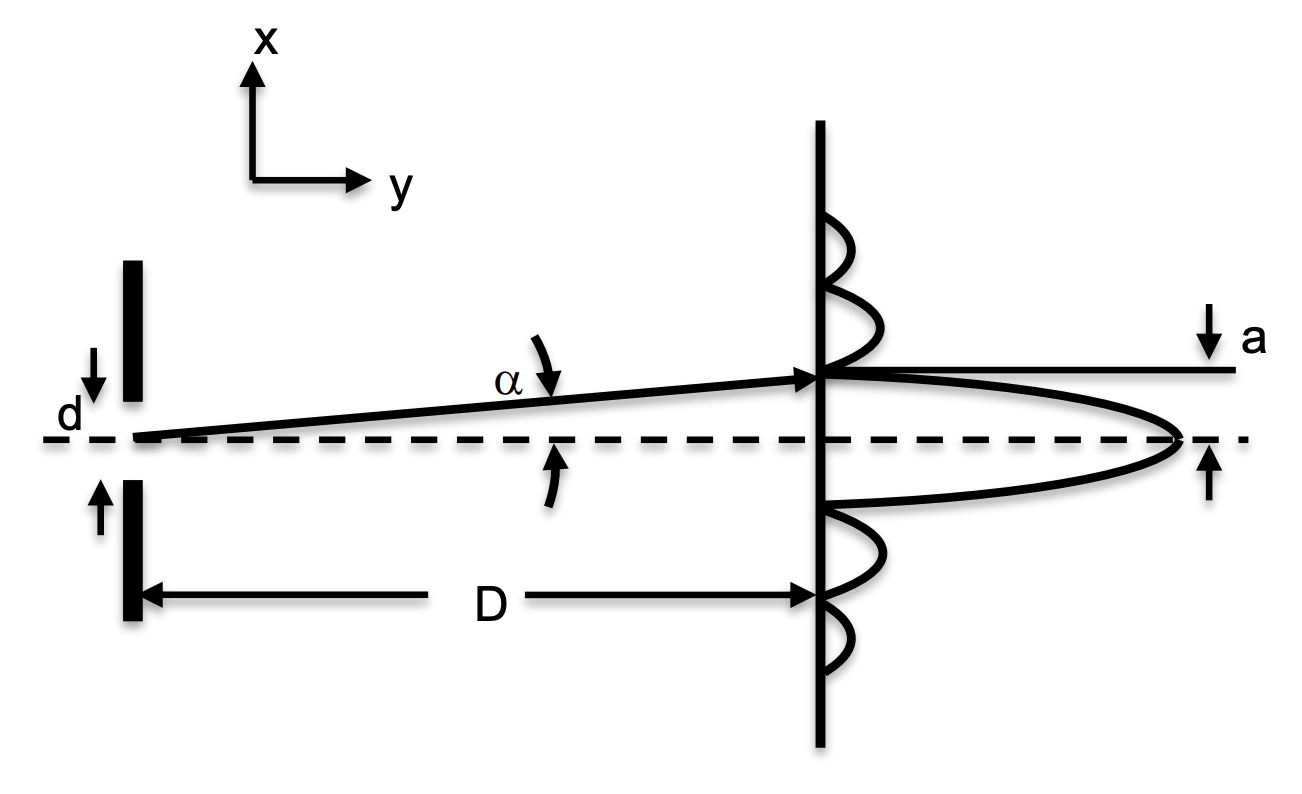
\includegraphics[width=0.8\textwidth]{../Figures/geometricdiagram.png}
    \caption{Geometric diagram of the single slit diffraction experiment. The slit width is denoted as w,
    the angle to the first minima is denoted as $\alpha$ and the distance from the maximum intensity to the 
    first minima is denoted as $a$. The distance from the observation plane to the diffraction plane will be 
    denoted as $L$.}
    \label{fig:geometricdiagram}
\end{figure}

From Figure \ref{fig:geometricdiagram}, photons passing through the slit have an uncertainty in the x direction 
equal to the width of the slit, as the photons cannot exist outside this range,

\begin{equation*}
    \Delta x = w/2.
\end{equation*}

The uncertainty of the photon's velocity in the x-direction is given by the relation, using trigonometry,

\begin{equation*}
    \Delta v_x = c\sin{\alpha}.
\end{equation*}

Therefore the uncertainty in momentum of the photon in the x direction is 

\begin{equation*}
    \Delta p_x = mc\sin{\alpha}.
\end{equation*}

Using the de Broglie relation $p=\frac{h}{\lambda}$,

\begin{equation*}
    \Delta p_x = \frac{h}{\lambda}\sin{\alpha}.
\end{equation*}

Recall that $\sin{\alpha} \approx \frac{\lambda}{w}$,

\begin{equation*}
    \Delta p_x = \frac{h}{w},
\end{equation*}

and so we can obtain 

\begin{equation*}
    \Delta x \Delta p_x = h/2.
\end{equation*}

We can now write, using Figure \ref{fig:geometricdiagram},

\begin{equation*}
    \Delta p_x = \frac{h}{\lambda}\sin\left(\tan^{-1}{\frac{a}{L}}\right),
\end{equation*}

using Heisenberg's uncertainty principle,

\begin{equation*}
    \Delta x \Delta p_x \geq \frac{\hbar}{2},
\end{equation*}

our expression becomes

\begin{equation*}
    \Delta x \Delta p_x = \frac{wh}{2\lambda}\sin\left(\tan^{-1}{\frac{a}{L}}\right) \geq \frac{\hbar}{2}.
\end{equation*}

Or equivalently,

\begin{equation} \label{eqn:HUP}
    \frac{2\pi w}{\lambda}\sin\left({\tan^{-1}{\frac{a}{L}}}\right) \geq 1.
\end{equation}

\subsection{Experimental Setup}
The single slit in front of the detector will convolve the incoming intensity from the diffracted field, i.end

\begin{equation*}
    I_{\text{measured}}(x) = I_{\text{field}}(x) * \prod_{-\frac{1}{2}+\frac{1}{2}}\left(\frac{x}{w}\right)
\end{equation*}

where $x$ is the horizontal translation of the single slit and the detector as it scans the diffracted field along 
the observation plane. Decreasing the width of the single slit will improve uncertainty in position so $\Delta x$ 
decreases and improves resolution in smaller features however there will be loss of information as intensity of light 
decreases.

Since we want to convolve two functions, we need to convert our diffracted field intensity into a function of the lateral 
distance on the observation plane. Using trigonometry and a small angle approximation, we can say that 

\begin{equation*}
    \sin{\theta} \approx \tan{\theta} \approx \theta = \frac{x}{L},
\end{equation*}

where $L$ is the distance from the single slit to the observation plane. However, since we are taking multiple measured intensities,
the resulting pattern should resemble the original diffraction intensity field,

\begin{equation}\label{eqn:Ifield}
    I_{\text{field}}(x) = \sum_{i}I_{\text{measured}}(x) = w^2\left(\frac{\sin\left(\pi w \frac{x}{\lambda L}\right)}{\pi w \frac{x}{\lambda L}}\right)^2
\end{equation}

The distance from the aperture plane to the observation plane is measured to be $117 \pm 0.25$ cm. The wavelength of the laser is $632.8$ nm.

\subsubsection{Fitted function}
The curve fits for the theoretical results were done in two ways. The first method was to just simply take Equation \ref{eqn:Ifield} and 
plug in the physical parameters. The controlled physical parameters are the length of the aperture plane to the observation plane, the wavelength of the
laser whilst the width of the slit is the variable being changed. Hence, we can just simply find the idealised theoretical model, assuming these 
controlled variables are exactly what the specifications state. The second method of fitting a theoretical curve is to use scipy.optimize's curvefit function.
A simplified version of Equation \ref{eqn:Ifield} was defined,

\begin{equation*}
    I_{\text{fitted}} = \text{sinc}(k\pi x)^2
\end{equation*}

where $k$ is the fitting parameter. In theory, $k$ contains all the information about the width, wavelength of laser and the optical length however, we can abstract 
it away and let scipy.optimize find the best fitting value. From this fit, we are also able to find an uncertainty value, equal to the average least squared deviation of the 
experimental values to the theoretical fit.

\section{Results \& Analysis}

\subsection{0.1 mm slit}

\begin{figure}[H]
    \centering
    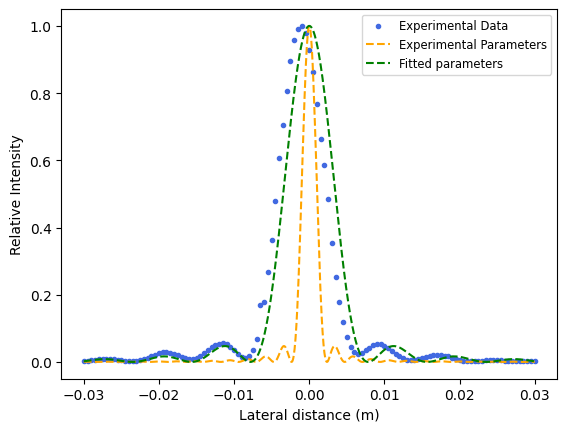
\includegraphics[width=0.6\textwidth]{../Figures/0_1mm.png}
    \caption{Plot of the intensity of the diffracted field over the lateral distance on the observation plane for the 0.1 mm slit. The experimental data is displayed as 
    blue dots. In the range away from the peak, the data points are relatively close enough together to create a continuous curve. Towards the peak, 
    the data points are further apart. In the case of using the 0.1 mm slit, the peak intensity is defined well enough to induce confidence in modelling 
    the data with a sinc function. The fitted curve is shown as the dotted green line whilst the function using experimental parameters is shown as the 
    dotted yellow line. Experimentally, the minima lie at -0.0235, -0.0155, -0.0085, 0.0065, 0.0135, 0.0215 and 0.0275 m. However, for calculations, we 
    will be using the minima obtained from the fitted curve. These minima lie at -0.0235, -0.0157, -0.0078, 0.0078, 0.0157 and 0.0235 m. The uncertainty 
    of the fitted curve is 2.5\%.}
    \label{fig:0_1}
\end{figure}

We can first find the angle to the minima, $\alpha$ and compare with results in the previous section. From Figure \ref{fig:0_1}, we find that $a=0.0078 \pm 0.0002$ m. Thus,

\begin{align*}
    \alpha &= \tan^{-1}\frac{a}{L} \\
    &= \tan^{-1}\frac{0.0078}{1.17} \\
    &= 0.384 \pm 0.01^\circ
\end{align*}

The expected diffraction angles for the 0.1 mm slit was $\alpha = 0.363^\circ$ and so the experimental value disagrees with the theoretical value. This 
could be due to the small angle approximation made earlier for Equation \ref{eqn:minima}. We can also check for the second order minima angle as we have 
the distance from the second order minima to the central maximum being 0.0157 m. Using trigonometry again, we find that the experimental angle is found 
to be $\theta = 0.769 \pm 0.02^\circ$. Again this does not agree with the thereotical value of $0.0725^\circ$, suggesting some systematic uncertainty we have 
not accounted for.

To check Equation \ref{eqn:HUP}, we can substitute our value of $a$ and $w$, 

\begin{align*}
    \Delta x \Delta p_x &= \frac{2\pi w}{\lambda} \sin\left(\tan^{-1}\frac{a}{L}\right) \\ 
    &= \frac{2\pi (0.1 \times 10^{-3})}{(632.8 \times 10^{-9})}\sin\left(\tan^{-1}\frac{(0.0078)}{(117\times10^{-2})}\right) \\
    &= 6.65 \\
    &\geq 1.
\end{align*}

Therefore, the Heisenberg Uncertainty principle is upheld in the case of the diffraction pattern from a 0.1 mm slit.

\subsection{0.2 mm slit}

\begin{figure}[H]
    \centering
    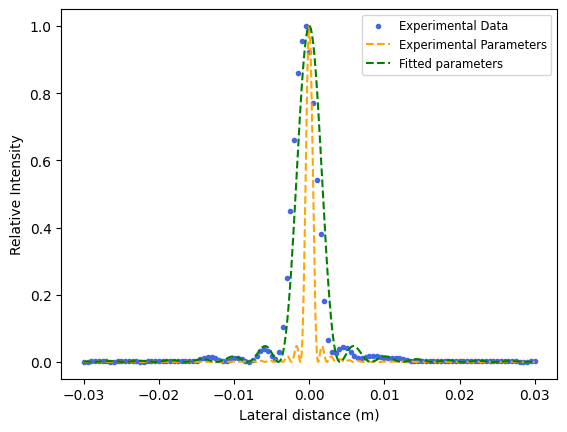
\includegraphics[width=0.475\textwidth]{../Figures/0_2mm.png}
    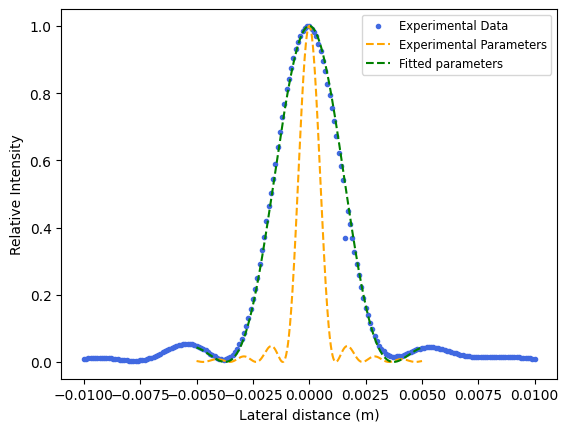
\includegraphics[width=0.475\textwidth]{../Figures/0_2mmv2.png}
    \caption{Same plot as in the figure above but for the 0.2 mm slit. (a) Intensity field scanned in increments of 1 mm. The experimental data (blue) get quite sparse near 
    the peak. The uncertainty of the fitted parameters is 2.7\%. We can improve this as seen in the plot on the right. (b) Intensity field scanned 
    in increments of 0.2 mm. The uncertainty reduces down to 0.3\% for the fitted curve (green). The minima given by the fitted curve are -0.00374 and 0.00374 m.}
    \label{fig:0_2}
\end{figure}

We can first compare the expected first diffracted angle to the experimentally obtained one. Beginning with Equation \ref{eqn:minima}, we find that the theoretical angle 
should be 

\begin{equation*}
    \alpha_{\text{Theoretical}} = 0.181^\circ.
\end{equation*}

Experimentally, the angle can be calculated by taking the inverse tan ratio of the $a$ value of 0.00374 and $L$, gives us,

\begin{equation*}
    \alpha_{\text{Experimental}} = 0.183^\circ
\end{equation*}

where the uncertainty is negligible due to the ridiculous small uncertainty given by the fitted parameters and the uncertainty in the length measurement. Again, we find that 
the theoretical and experimental values do not agree with each other.

The Heisenberg Uncertainty is then,

\begin{align*}
    \Delta x \Delta p_x &= \frac{2 \pi w}{\lambda}\sin{\left(\tan^{-1}\frac{a}{L}\right)} \\
    &= \frac{2\pi \times 0.2\times10^{-3}}{632.8\times10^{-9}}\sin{\left(\tan^{-1}\frac{0.00374}{117\times 10^{-2}}\right)} \\
    &= 6.348 \\
    &\geq 1.
\end{align*}

Therefore, again, the Heisenberg Uncertainty principle is satisfied in the case of the diffraction pattern produced by the 0.2 mm slit.

\subsection{0.4 mm slit}

\begin{figure}[H]
    \centering
    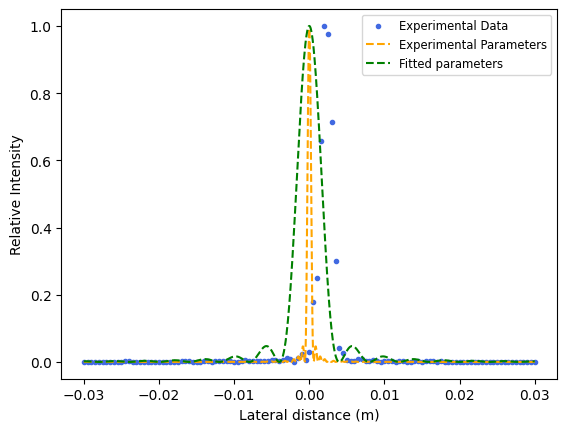
\includegraphics[width=0.475\textwidth]{../Figures/0_4mm.png}
    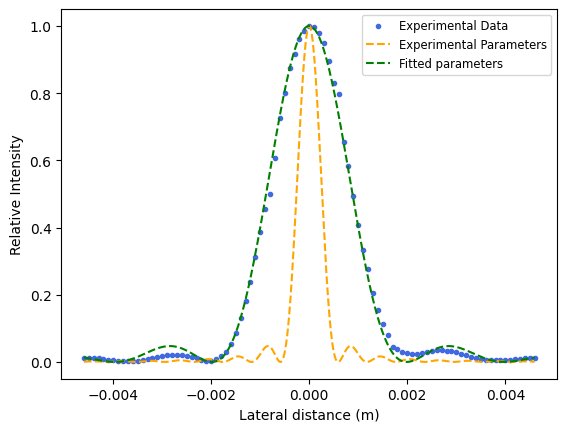
\includegraphics[width=0.475\textwidth]{../Figures/0_4mmv2.png}
    \caption{Exact same plot as the figures above but for the 0.4 mm slit. (a) Intensity field scanned in increments of 1 mm. The experimental data (blue) is even worse than 
    in the 0.2 mm case, infact since the experimental data is so sparse near the central maximum, the fitted curve (green) is completely off. The uncertainty produced is 10\%. (b)
    The intensity field is now scanned in increments of 0.2 mm. The uncertainty improves to 0.5\% and the central maximum is more clearly defined, allowing for the fitted 
    parameters to be more certain. The minima given by the fitted curve are -0.00397, -0.00198, 0.00198 and 0.00397 m.}
    \label{fig:0_4}
\end{figure}

We will again check for the expected first minima angle and the experimentally obtained value. Repeating our analysis for the 0.1 mm and 0.2 mm, we find that the theoretical 
minima angle to be

\begin{equation*}
    \alpha_{\text{Theoretical}} = 0.0906^\circ. 
\end{equation*}

Our experimentally value is then 

\begin{equation*}
    \alpha_{\text{Experimental}} = 0.0972^\circ.
\end{equation*}

Again the uncertainty is insignificant so is disregarded here.

Finally checking the uncertainty principle, 

\begin{align*}
    \Delta x \Delta p_x &= \frac{2 \pi w}{\lambda}\sin{\left(\tan^{-1}\frac{a}{L}\right)} \\
    &= \frac{2\pi \times 0.4\times10^{-3}}{632.8\times10^{-9}}\sin{\left(\tan^{-1}\frac{0.001984}{117\times 10^{-2}}\right)} \\
    &= 6.737 \\
    &\geq 1.
\end{align*}

Again, we find that the Heisenberg Uncertainty principle is satisfied for the diffraction pattern for the 0.4 mm slit as well.

\section{Discussion}

We found that for diffraction patterns for a single slit aperture of width 0.1, 0.2 and 0.4 mm all obey Heisenberg Uncertainty principle and follow 
the predictions made by quantum mechanics. This was tested to a high degree of accuracy as the uncertainties for each experiment was 2.5\%, 0.5\% and 
0.3\% respectively. However, if we take a look at the expected angle of the first minima for all 3 patterns versus the experimentally obtained values,
there is an unexplained discrepancy. This is related to the sinc function (yellow dotted line) fitted with experimental parameters shown in Figures 
\ref{fig:0_1}, \ref{fig:0_2} and \ref{fig:0_4}. This systematic uncertainty is likely due to unideal assumptions such as the monochromatic and coherent 
nature of light. In reality, perflectly coherent light does not exist so the assumption for Fraunhofer diffraction is not applicable in the real world.
There are also other limitations such as quality and degradation of equipment. Lasers also do not emit perfect plane waves or a uniform beam which is a 
key assumption of scalar diffraction. There are also systematic uncertainties that are hard to or almost impossible to quantify or observe such as the 
imperfections in the slit or the alignment of the whole set up not being perfect. Nevertheless, all these imperfections would contribute to the expected 
curve being much thinner in width than our experimentally obtained curves.

\section{Conclusion}

We verified Heisenberg's Uncertainty principle in the case of predicted inequalities in a diffraction field from a single slit. We used single slits of width 
0.1 mm, 0.2 mm and 0.4 mm and found that for all 3 experiments, the inequality predicted by quantum mechanics holds true. 

\section{Appendix}
\subsection{Similar Experiment}
The diffracted angles in Question 2 were given by

\begin{equation*}
    \theta = \frac{n \lambda}{w}.
\end{equation*}

Using de Broglie relation,

\begin{equation*}
    p = \frac{h}{\lambda} = mv,
\end{equation*}

We can rearrange for $\lambda$,

\begin{equation*}
    \lambda = \frac{h}{mv}.
\end{equation*}

This allows us to rewrite the initial equation as 

\begin{equation*}
    \theta = \frac{n h}{w m v},
\end{equation*}

we want to keep $\theta$ and n as consistent as before so, 

\begin{equation*}
    \frac{h}{wmv} = \frac{632.8\times10^{-9}}{0.1\times10^{-3}},
\end{equation*}

rearranging for the width of the slit,

\begin{equation*}
    w = \frac{h(0.1\times10^{-3})}{mv(632.8\times10^{-9})}
\end{equation*}

For part (a), $m_e=9.109\times10^{-31}$ kg and $v=0.15c$,

\begin{equation*}
    w = 2.55\times10^{-9} \text{ m}.
\end{equation*}

For an $n$ number of electrons,

\begin{equation*}
    w_n = \frac{2.55\times10^{-9}}{n}
\end{equation*}

For part (b), $m=7.21\times10^{-26}$ kg per molecule and $v=220$ ms$^{-1}$,

\begin{equation*}
    w_n = \frac{6.60\times10^{-9}}{n} \text{ m}
\end{equation*}

for n molecules.

\subsection{Lab book}

\begin{figure}
    \centering
    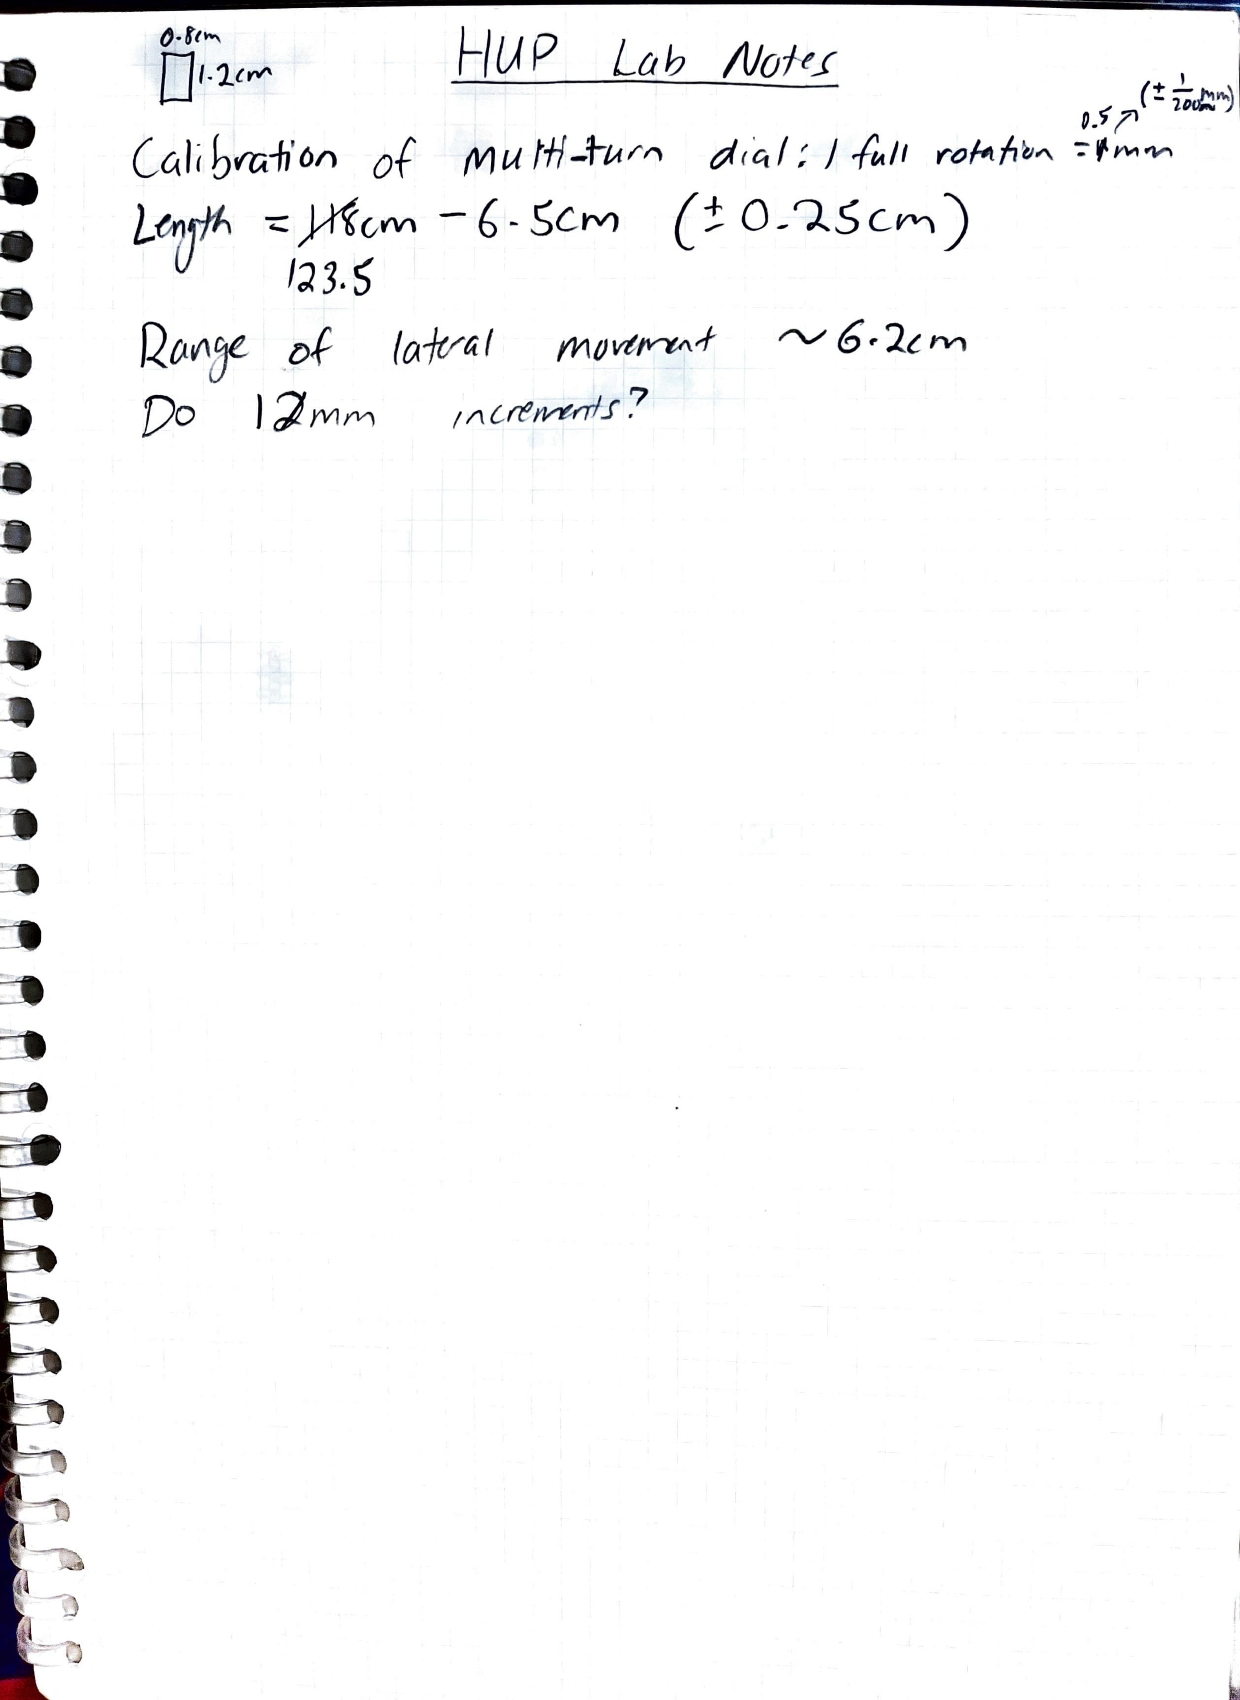
\includegraphics[width=0.8\textwidth]{../Figures/labbook.jpg}
\end{figure}

\end{document}